%-------------------------------------------------------------------------------------------------------------------------------------------------------------------------------------------------
% Section 3
%
%-------------------------------------------------------------------------------------------------------------------------------------------------------------------------------------------------
\section{Properties of Bernoulli line ensembles}\label{Section3} In this section we derive several results for Bernoulli line ensembles, which will be used in the proof of Theorem \ref{PropTightGood} in Section \ref{Section4}.


%-------------------------------------------------------------------------------------------------------------------------------------------------------------------------------------------------
% Section 3.1
%
%-------------------------------------------------------------------------------------------------------------------------------------------------------------------------------------------------
\subsection{Monotone coupling lemmas}\label{Section3.1}
 In this section we formulate two lemmas that provide couplings of two Bernoulli line ensembles of non-intersecting Bernoulli bridges on the same interval, which depend monotonically on their boundary data. Schematic depictions of the couplings are provided in Figure \ref{fig:MCL}. We postpone the proof of these lemmas until Section \ref{Section8}. 
\begin{figure}[ht]
  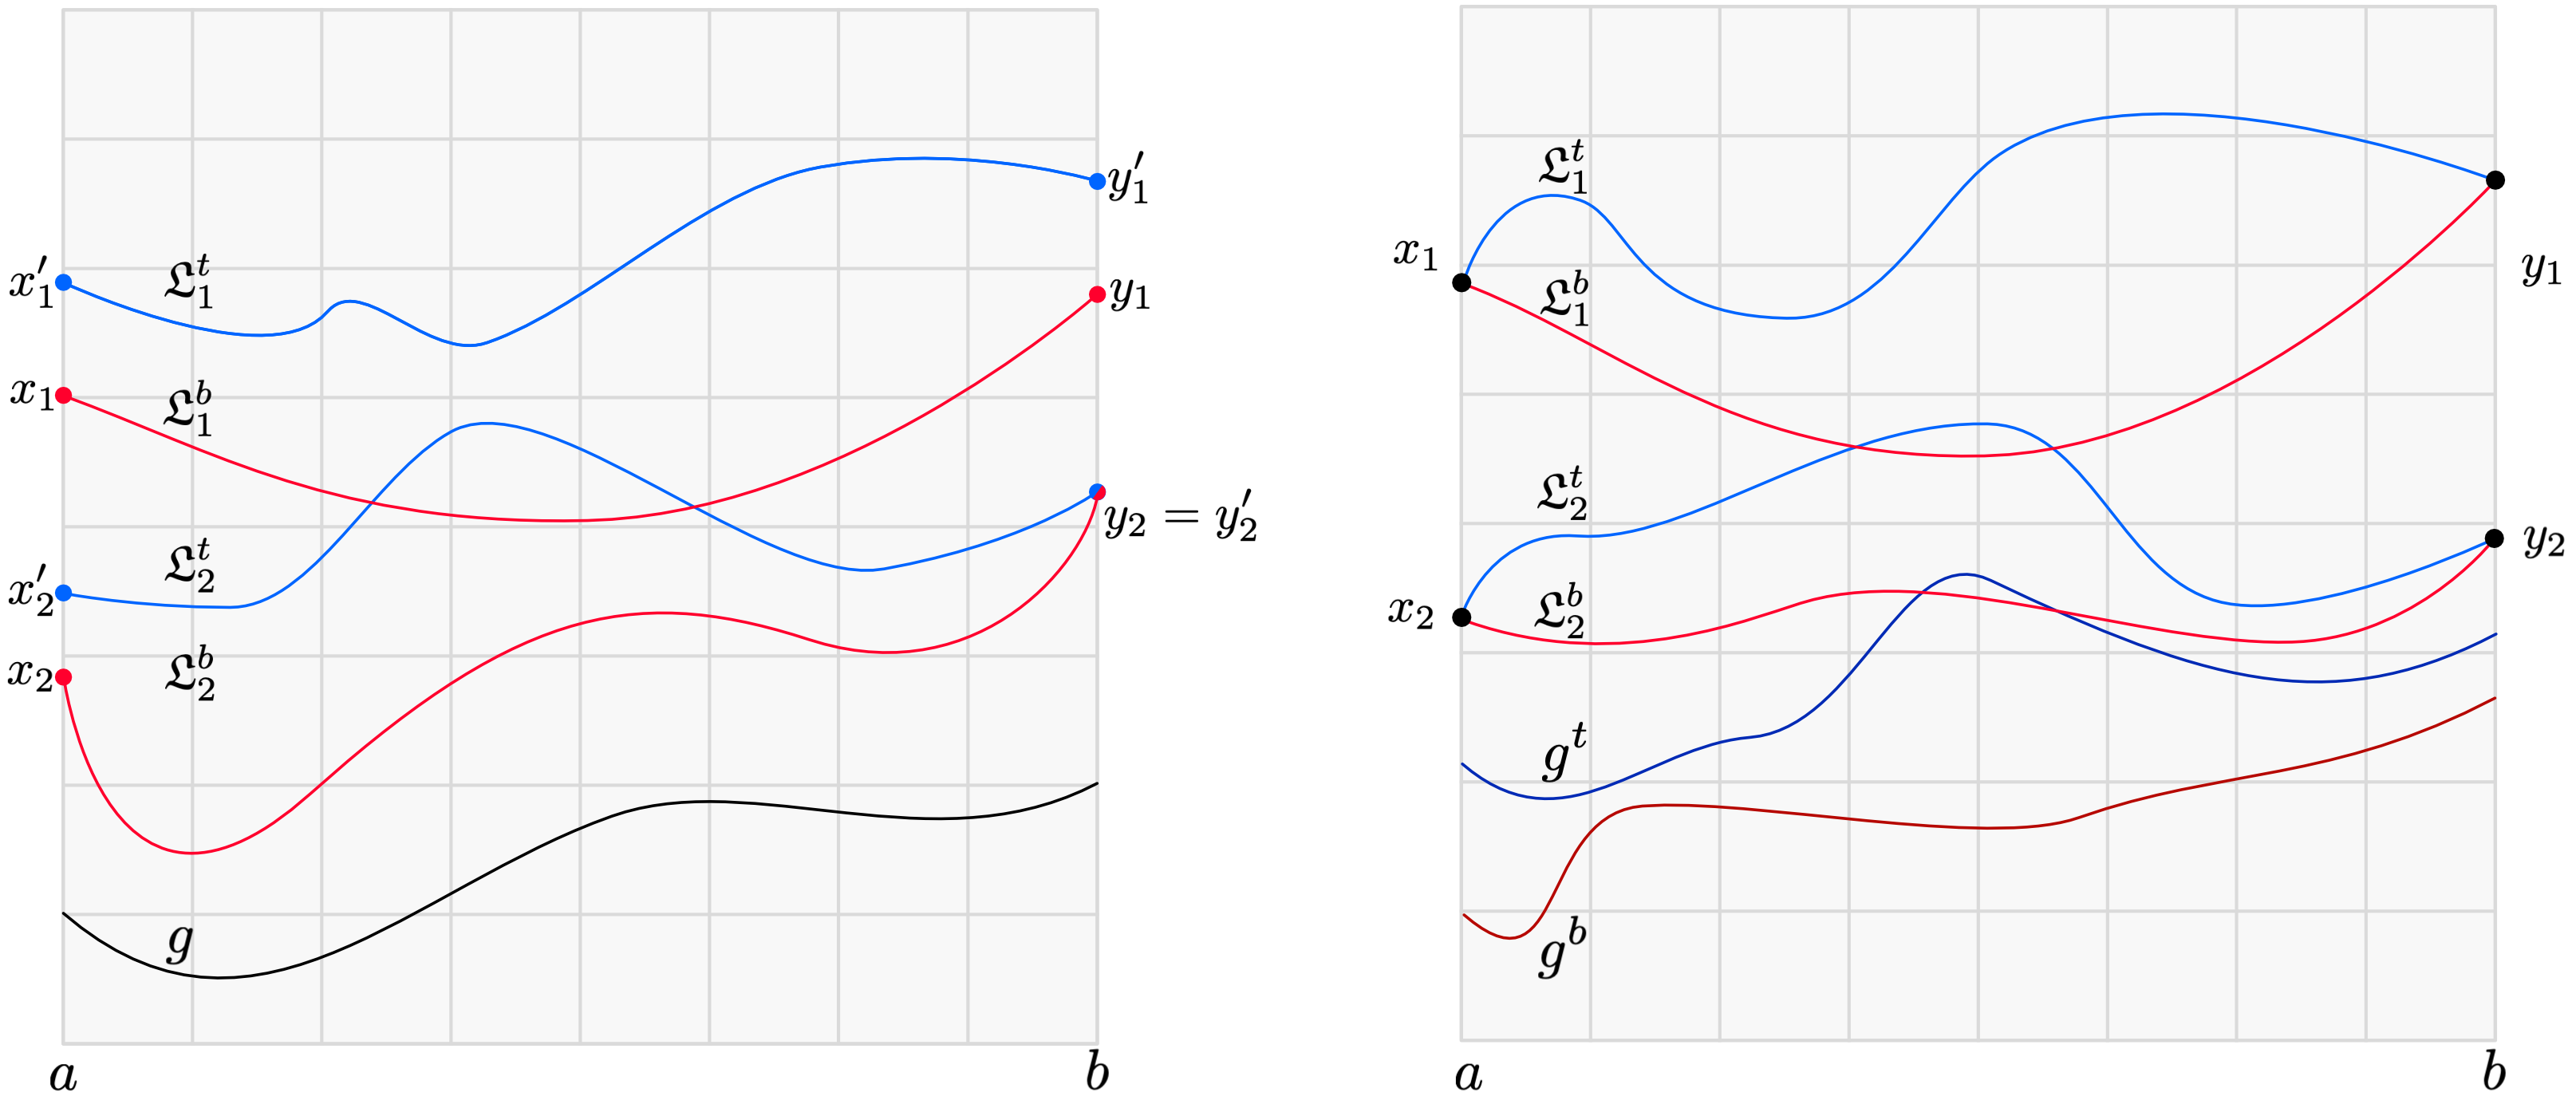
\includegraphics[width=1.02\textwidth]{graphics/MonotoneCoupling.png}
  \caption{Two diagrammatic depictions of the monotone coupling Lemma \ref{MCLxy} (left part) and Lemma \ref{MCLfg} (right part). Red depicts the lower line ensemble and accompanying entry data, exit data, and bottom bounding curve, while blue depicts that of the higher ensemble.}
  \label{fig:MCL}
\end{figure}

\begin{lemma}\label{MCLxy} Assume the same notation as in Definition \ref{DefAvoidingLawBer}. Fix $k \in \mathbb{N}$, $T_0, T_1 \in \mathbb{Z}$ with $T_0 < T_1$, $S\subseteq\llbracket T_0,T_1\rrbracket$, a function $g: \llbracket T_0, T_1 \rrbracket  \rightarrow [-\infty, \infty)$ as well as $\vec{x}, \vec{y}, \vec{x}\,', \vec{y}\,' \in \mathfrak{W}_k$. Assume that $\Omega_{avoid}(T_0, T_1, \vec{x}, \vec{y}, \infty,g; S)$ and $\Omega_{avoid}(T_0, T_1, \vec{x}', \vec{y}', \infty,g; S)$ are both non-empty. Then there exists a probability space $(\Omega, \mathcal{F}, \mathbb{P})$, which supports two $\llbracket 1, k \rrbracket$-indexed Bernoulli line ensembles $\mathfrak{L}^t$ and $\mathfrak{L}^b$ on $\llbracket T_0, T_1 \rrbracket$ such that the law of $\mathfrak{L}^{t}$ {\big (}resp. $\mathfrak{L}^b${\big )} under $\mathbb{P}$ is given by $\mathbb{P}_{avoid, Ber; S}^{T_0, T_1, \vec{x}\,', \vec{y}\,', \infty, g}$ {\big (}resp. $\mathbb{P}_{avoid, Ber; S}^{T_0, T_1, \vec{x}, \vec{y}, \infty, g}${\big )} and such that $\mathbb{P}$-almost surely we have $\mathfrak{L}_i^t(r) \geq \mathfrak{L}^b_i(r)$ for all $i = 1,\dots, k$ and $r \in \llbracket T_0, T_1 \rrbracket$.
\end{lemma}

\begin{lemma}\label{MCLfg} Assume the same notation as in Definition \ref{DefAvoidingLawBer}. Fix $k \in \mathbb{N}$,  $T_0, T_1 \in \mathbb{Z}$ with $T_0 < T_1$, $S\subseteq\llbracket T_0, T_1\rrbracket$, two functions $g^t, g^b: \llbracket T_0, T_1 \rrbracket \rightarrow [-\infty,\infty)$ and $\vec{x}, \vec{y} \in \mathfrak{W}_k$. We assume that $g^t(r) \geq g^b(r)$ for all $r \in \llbracket T_0, T_1 \rrbracket$ and that $\Omega_{avoid}(T_0, T_1, \vec{x}, \vec{y}, \infty,g^t; S)$ and $\Omega_{avoid}(T_0, T_1, \vec{x}, \vec{y}, \infty,g^b; S)$ are both non-empty. Then there exists a probability space $(\Omega, \mathcal{F}, \mathbb{P})$, which supports two $\llbracket 1, k \rrbracket$-indexed Bernoulli line ensembles $\mathfrak{L}^t$ and $\mathfrak{L}^b$ on $\llbracket T_0, T_1 \rrbracket$ such that the law of $\mathfrak{L}^{t}$ {\big (}resp. $\mathfrak{L}^b${\big )} under $\mathbb{P}$ is given by $\mathbb{P}_{avoid, Ber; S}^{T_0, T_1, \vec{x}, \vec{y}, \infty, g^t}$ {\big (}resp. $\mathbb{P}_{avoid, Ber; S}^{T_0,T_1, \vec{x}, \vec{y}, \infty, g^b}${\big )} and such that $\mathbb{P}$-almost surely we have $\mathfrak{L}_i^t(r) \geq \mathfrak{L}^b_i(r)$ for all $i = 1,\dots, k$ and $r \in \llbracket T_0, T_1 \rrbracket$.
\end{lemma}

In plain words, Lemma \ref{MCLxy} states that one can couple two Bernoulli line ensembles $\mathfrak{L}^{t}$ and $\mathfrak{L}^{b}$ of non-intersecting Bernoulli bridges, bounded from below by the same function $g$, in such a way that if all boundary values of $\mathfrak{L}^{t}$ are above the respective boundary values of $\mathfrak{L}^{b}$, then all up-right paths of $\mathfrak{L}^{t}$ are almost surely above the respective up-right paths of $\mathfrak{L}^{b}$. See the left part of Figure \ref{fig:MCL}. Lemma \ref{MCLfg}, states that one can couple two Bernoulli line ensembles $\mathfrak{L}^{t}$ and $\mathfrak{L}^{b}$ that have the same boundary values, but the lower bound $g^t$ of $\mathfrak{L}^{t}$ is above the lower bound $g^b$ of $\mathfrak{L}^{b}$, in such a way that all up-right paths of $\mathfrak{L}^{t}$ are almost surely above the respective up-right paths of $\mathfrak{L}^{b}$. See the right part of Figure \ref{fig:MCL}.


%-------------------------------------------------------------------------------------------------------------------------------------------------------------------------------------------------
% Section 3.2
%
%-------------------------------------------------------------------------------------------------------------------------------------------------------------------------------------------------
\subsection{Properties of Bernoulli bridges}\label{Section3.2} In this section we derive several results about Bernoulli bridges, which are random up-right paths that have law $\mathbb{P}_{Ber}^{T_0, T_1, x,y}$ as in Section \ref{Section2.2}. Our results will rely on the two monotonicity Lemmas \ref{MCLxy} and \ref{MCLfg} as well as a strong coupling between Bernoulli bridges and Brownian bridges from \cite{CD} -- recalled here as Theorem \ref{KMT}.

If $W_t$ denotes a standard one-dimensional Brownian motion and $\sigma > 0$, then the process
$$B^{\sigma}_t = \sigma (W_t - t W_1), \hspace{5mm} 0 \leq t \leq 1,$$
is called a {\em Brownian bridge (conditioned on $B_0 = 0, B_1 = 0$) with variance $\sigma^2$.} We note that $B^\sigma$ is the unique a.s. continuous Gaussian process on $[0,1]$ with $B_0 = B_1  = 0$, $\ex[B^\sigma_t] = 0$, and
\begin{equation}\label{BBcovar}
\ex[B^\sigma_r B^\sigma_s] = \sigma^2(r\wedge s - rs - sr + sr) = \sigma^2 (r\wedge s - rs).
\end{equation}  
With the above notation we state the strong coupling result we use.
\begin{theorem}\label{KMT}
Let $p \in (0,1)$. There exist constants $0 < C, a, \alpha < \infty$ (depending on $p$) such that for every positive integer $n$, there is a probability space on which are defined a Brownian bridge $B^\sigma$ with variance $\sigma^2 = p(1-p)$ and a family of random paths $\ell^{(n,z)} \in \Omega(0,n, 0, z)$ for $z = 0,\dots,n$ such that $\ell^{(n,z)}$ has law $\mathbb{P}^{0,n,0,z}_{Ber}$ and
\begin{equation}\label{KMTeq}
\mathbb{E}\left[ e^{a \Delta(n,z)} \right] \leq C e^{\alpha (\log n)^2}e^{|z- p n|^2/n}, \mbox{ where $\Delta(n,z):=  \sup_{0 \leq t \leq n} \left| \sqrt{n} B^\sigma_{t/n} + \frac{t}{n}z - \ell^{(n,z)}(t) \right|.$}
\end{equation}
\end{theorem}
\begin{remark} When $p = 1/2$ the above theorem follows (after a trivial affine shift) from \cite[Theorem 6.3]{LF} and the general $p \in (0,1)$ case was done in \cite[Theorem 4.5]{CD}. We mention that a significant generalization of Theorem \ref{KMT} for general random walk bridges has recently been proved in \cite[Theorem 2.3]{DW19}.
\end{remark}

We will use the following simple corollary of Theorem \ref{KMT} to compare Bernoulli bridges with Brownian bridges. We use the same notation as in the theorem.

\begin{corollary}\label{Cheb}
	Fix $p\in (0,1)$, $\beta > 0$, and $A>0$. Suppose $|z-pn| \leq K\sqrt{n}$ for a constant $K>0$. Then for any $\epsilon > 0$, there exists $N$ large enough depending on $p,\epsilon,A,K$ so that for $n\geq N$,
	\[
	\mathbb{P}\Big(\Delta(n,z) \geq An^\beta\Big) < \epsilon.
	\]
\end{corollary}

\begin{proof}
	Applying Chebyshev's inequality and \eqref{KMTeq} gives
	\begin{align*}
	\mathbb{P}\Big(\Delta(n,z) \geq An^\beta\Big) &\leq e^{-An^\beta}\ex\Big[e^{a\Delta(n,z)}\Big] \leq C\exp\Big[-An^\beta + \alpha(\log n)^2 + \frac{|z-pn|^2}{n}\Big]\\
	&\leq C\exp\Big[-An^\beta + \alpha(\log n)^2 + K\Big].
	\end{align*}
	The conclusion is now immediate.
\end{proof}

We also state the following result regarding the distribution of the maximum of a Brownian bridge, which follows from formulas in \cite[Chapter 12]{Dudley}.

\begin{lemma}\label{BBmax}
	Fix $p\in (0,1)$, and let $B^\sigma$ be a Brownian bridge of variance $\sigma^2 = p(1-p)$ on $[0,1]$. Then for any $C,T> 0$ we have
	\begin{equation}\label{BBmaxeq}
	\begin{split}
	\mathbb{P}\left(\max_{s\in[0,T]} B^\sigma_{s/T} \geq C\right) &= \exp\left( - \frac{2C^2}{p(1-p)}\right), \\ \mathbb{P}\left(\max_{s\in[0,T]} \big| B^\sigma_{s/T} \big| \geq C\right) &= 2\sum_{n=1}^\infty (-1)^{n-1} \exp\left(-\frac{2n^2C^2}{p(1-p)}\right).
	\end{split}
	\end{equation}
	In particular,
	\begin{equation}\label{sepBd}
	\mathbb{P}\left(\max_{s\in[0,T]} \big|B^\sigma_{s/T}\big| \geq C\right) \leq 2\exp\left( - \frac{2C^2}{p(1-p)}\right).
	\end{equation}
\end{lemma}

\begin{proof}
	Let $B^1$ be a Brownian bridge with variance 1 on $[0,1]$. Then $B^\sigma_t$ has the same distribution as $\sigma B^1_t$. Hence
	\begin{equation*}
	\mathbb{P}\left( \max_{s\in[0,T]} B^\sigma_{s/T} \geq C \right) = \mathbb{P}\left( \max_{t\in[0,1]} B^1_t \geq C/\sigma \right) = e^{-2(C/\sigma)^2} = e^{-2C^2/p(1-p)}.
	\end{equation*}
	The second equality follows from \cite[Proposition 12.3.3]{Dudley}. This proves the first equality in \eqref{BBmaxeq}. Similarly, using \cite[Proposition 12.3.4]{Dudley} we find
	\begin{equation*}
	\mathbb{P}\left( \max_{s\in[0,T]} \big| B^\sigma_{s/T}\big| \geq C \right) = \mathbb{P}\left( \max_{t\in[0,1]} \big| B^1_t\big| \geq C/\sigma \right) = 2\sum_{n=1}^\infty (-1)^{n-1}e^{-2n^2C^2/\sigma^2},
	\end{equation*}
	proving the second inequality in \eqref{BBmaxeq}.
	
	Lastly to prove \eqref{sepBd}, observe that since $B^\sigma_t$ has mean 0, $B^\sigma_t$ and $-B^\sigma_t$ have the same distribution. It follows from the first equality above that
	\begin{equation*}
	\begin{split}
	&\mathbb{P}\left( \max_{s\in[0,T]} \big| B^\sigma_{s/T}\big| \geq C \right) \leq \mathbb{P}\left( \max_{s\in[0,T]}  B^\sigma_{s/T} \geq C \right) + \mathbb{P}\left( \max_{s\in[0,T]}  \big(-B^\sigma_{s/T}\big) \geq C \right) = \\
	&2\,\mathbb{P}\left( \max_{s\in[0,T]}  B^\sigma_{s/T} \geq C \right) = 2e^{-2C^2/p(1-p)}.
	\end{split}
	\end{equation*}
\end{proof}

We state one more lemma about Brownian bridges, which allows us to decompose a bridge on $[0,1]$ into two independent bridges with Gaussian affine shifts meeting at a point in $(0,1)$.

\begin{lemma}\label{2bridges}
	Fix $p\in (0,1)$, $T>0$, $t\in(0,T)$, and let $B^\sigma$ be a Brownian bridge of variance $\sigma^2 = p(1-p)$ on $[0,1]$. Let $\xi$ be a Gaussian random variable with mean 0 and variance
	\[
	\ex[\xi^2] = \sigma^2\frac{t}{T}\left(1-\frac{t}{T}\right).
	\]
	Let $B^1,B^2$ be two independent Brownian bridges on $[0,1]$ with variances $\sigma^2 t/T$ and $\sigma^2(T-t)/T$ respectively, also independent from $B^\sigma$. Define the process
	\[
	\tilde{B}_{s/T} = \begin{dcases}
	\frac{s}{t}\,\xi + B^1\Big(\frac{s}{t}\Big), & s\leq t,\\
	\frac{T-s}{T-t}\,\xi + B^2\Big(\frac{s-t}{T-t}\Big), & s\geq t,
	\end{dcases}
	\]
	for $s\in [0,T]$. Then $\tilde{B}$ is a Brownian bridge with variance $\sigma$.
\end{lemma}

\begin{proof}
	It is clear that the process $\tilde{B}$ is a.s. continuous. Since $\tilde{B}$ is built from three independent zero-centered Gaussian processes, it is itself a zero-centered Gaussian process and thus completely characterized by its covariance. Consequently, to show that $\tilde{B}$ is a Brownian bridge of variance $\sigma^2$, it suffices to show by (\ref{BBcovar}) that if $0\leq r\leq s\leq T$ we have
	\begin{equation}\label{covar}
	\ex[\tilde{B}_{r/T}\tilde{B}_{s/T}] = \sigma^2 \frac{r}{T}\Big(1-\frac{s}{T}\Big).
	\end{equation}
	First assume $s\leq t$ Using the fact that $\xi$ and $B^1_\cdot$ are independent with mean 0, we find
	\begin{equation*}
	\begin{split}
	&\ex[\tilde{B}_{r/T}\tilde{B}_{s/T}] = \frac{rs}{t^2}\cdot\sigma^2\frac{t}{T}\Big(1-\frac{t}{T}\Big) + \sigma^2\frac{t}{T}\cdot\frac{r}{t}\Big(1-\frac{s}{t}\Big) =\\
	&\sigma^2\frac{r}{T}\Big(\frac{s}{t} - \frac{s}{T} + 1 - \frac{s}{t}\Big) = \sigma^2\frac{r}{T}\Big(1-\frac{s}{T}\Big).
	\end{split}
	\end{equation*}
	If $r\geq t$, we compute
	\begin{equation*}
	\begin{split}
	&\ex[\tilde{B}_{r/T}\tilde{B}_{s/T}] = \frac{(T-r)(T-s)}{(T-t)^2}\cdot\sigma^2\frac{t}{T}\Big( 1 - \frac{t}{T}\Big) + \sigma^2\frac{T-t}{T}\cdot\frac{r-t}{T-t}\Big( 1 - \frac{s-t}{T-t}\Big) =\\
	&\frac{\sigma^2(T-s)}{T(T-t)}\left(\frac{t(T-r)}{T} + r-t\right) = \frac{\sigma^2(T-s)}{T(T-t)}\cdot\frac{r(T-t)}{T} = \sigma^2\frac{r}{T}\Big(1-\frac{s}{T}\Big).
	\end{split}
	\end{equation*}
	If $r < t < s$, then since $\xi$, $B^1_\cdot$, and $B^2_\cdot$ are all independent, we have
	\[
	\ex[\tilde{B}_{r/T}\tilde{B}_{s/T}] = \frac{r}{t}\cdot\frac{T-s}{T-t}\cdot\sigma^2\frac{t(T-t)}{T^2} = \sigma^2\frac{r(T-s)}{T^2} = \sigma^2\frac{r}{T}\Big(1-\frac{s}{T}\Big).
	\]
	This proves \eqref{covar} in all cases.
\end{proof}

Below we list six lemmas about Bernoulli bridges. We provide a brief informal explanation of what each result says after it is stated. All six lemmas are proved in a similar fashion. For the first four lemmas one observes that the event whose probability is being estimated is monotone in $\ell$. This allows by Lemmas \ref{MCLxy} and \ref{MCLfg} to replace $x,y$ in the statements of the lemmas with the extreme values of the ranges specified in each. Once the choice of $x$ and $y$ is fixed one can use our strong coupling results, Theorem \ref{KMT} and Corollary \ref{Cheb}, to reduce each of the lemmas to an analogous one involving a Brownian bridge with some prescribed variance. The latter statements are then easily confirmed as one has exact formulas for Brownian bridges, such as Lemma \ref{BBmax}.\\

\begin{lemma}\label{LemmaHalfS4} Fix $p \in (0,1)$, $T \in \mathbb{N}$ and $x, y\in \mathbb{Z}$ such that $T \geq y-x \geq 0$, and suppose that $\ell$ has distribution $\mathbb{P}^{0,T,x,y}_{Ber}$. Let $M_1, M_2 \in \mathbb{R}$ be given. Then we can find $W_0 = W_0(p,M_2 - M_1) \in \mathbb{N}$ such that for $T \geq W_0$, $x \geq M_1 T^{1/2}$, $y \geq pT + M_2 T^{1/2}$ and $s \in [0,T]$ we have
\begin{equation}\label{halfEq1S4}
\mathbb{P}^{0,T,x,y}_{Ber}\left( \ell(s)  \geq \frac{T-s}{T} \cdot M_1 T^{1/2} + \frac{s}{T} \cdot \big(p T + M_2 T^{1/2}\big) - T^{1/4} \right) \geq \frac{1}{3}.
\end{equation}
\end{lemma}
\begin{remark}
If $M_1, M_2 = 0$ then Lemma \ref{LemmaHalfS4} states that if a Bernoulli bridge $\ell$ is started from $(0,x)$ and terminates at $(T,y)$, which are above the straight line of slope $p$, then at any given time $s \in [0,T]$ the probability that $\ell(s)$ goes a modest distance below the straight line of slope $p$ is upper bounded by $ 2/3$.
\end{remark}
\begin{proof}
	Define $A = \lfloor M_1T^{1/2}\rfloor$ and $B = \lfloor pT + M_2 T^{1/2}\rfloor$. Then since $A\leq x$ and $B\leq y$, it follows from Lemma 3.1 that there is a probability space with measure $\mathbb{P}_0$ supporting random variables $L_1$ and $L_2$, whose laws under $\mathbb{P}_0$ are $\mathbb{P}^{0,T,A,B}_{Ber}$ and $\mathbb{P}^{0,T,x,y}_{Ber}$ respectively, and $\mathbb{P}_0$-a.s. we have $L_1\leq L_2$. Thus
	\begin{equation}\label{HalfS4MC}
	\begin{split}
	&\mathbb{P}^{0,T,x,y}_{Ber}\left( \ell(s)  \geq \frac{T-s}{T} \cdot M_1 T^{1/2} + \frac{s}{T} \cdot \big(p T + M_2 T^{1/2}\big) - T^{1/4} \right) =\\
	& \mathbb{P}_0\left( L_2(s)  \geq \frac{T-s}{T} \cdot M_1 T^{1/2} + \frac{s}{T} \cdot \big(p T + M_2 T^{1/2}\big) - T^{1/4} \right) \geq\\
	&\mathbb{P}_0\left( L_1(s)  \geq \frac{T-s}{T} \cdot M_1 T^{1/2} + \frac{s}{T} \cdot \big(p T + M_2 T^{1/2}\big) - T^{1/4} \right) =\\
	&\mathbb{P}^{0,T,A,B}_{Ber}\left( \ell(s)  \geq \frac{T-s}{T} \cdot M_1 T^{1/2} + \frac{s}{T} \cdot \big(p T + M_2 T^{1/2}\big) - T^{1/4} \right).
	\end{split}
	\end{equation}
	Since the uniform distribution on upright paths on $\llbracket 0,T\rrbracket \times \llbracket A,B\rrbracket$ is the same as that on upright paths on $\llbracket 0,T\rrbracket \times \llbracket 0, B-A\rrbracket$ shifted vertically by $A$, the last line of \eqref{HalfS4MC} is equal to
	\[
	\mathbb{P}^{0,T,0,B-A}_{Ber}\left( \ell(s) + A  \geq \frac{T-s}{T} \cdot M_1 T^{1/2} + \frac{s}{T} \cdot \big(p T + M_2 T^{1/2}\big) - T^{1/4} \right).
	\]
	Now we employ the coupling provided by Theorem \ref{KMT}. We have another probability space $(\Omega,\mathcal{F},\mathbb{P})$ supporting a random variable $\ell^{(T,B-A)}$ whose law under $\mathbb{P}$ is $\mathbb{P}^{0,T,0,B-A}_{Ber}$ as well as a Brownian bridge $B^\sigma$ coupled with $\ell^{(T,B-A)}$. We have 
	\begin{equation}\label{HalfS4split}
	\begin{split}
	&\mathbb{P}^{0,T,0,B-A}_{Ber}\left( \ell(s) + A  \geq \frac{T-s}{T} \cdot M_1 T^{1/2} + \frac{s}{T} \cdot \big(p T + M_2 T^{1/2}\big) - T^{1/4} \right) =\\
	& \mathbb{P}\left( \ell^{(T,B-A)}(s) + A \geq \frac{T-s}{T} \cdot M_1 T^{1/2} + \frac{s}{T} \cdot \big(p T + M_2 T^{1/2}\big) - T^{1/4} \right) =\\
	& \mathbb{P}\bigg( \left[\ell^{(T,B-A)}(s) - \sqrt{T} B^\sigma_{s/T} - \frac{s}{T}\cdot(B-A)\right] + \sqrt{T}B^\sigma_{s/T} \geq \\
	&\qquad -A-\frac{s}{T}\cdot(B-A) +\frac{T-s}{T} \cdot M_1 T^{1/2} + \frac{s}{T} \cdot \big(p T + M_2 T^{1/2}\big) - T^{1/4} \bigg).
	\end{split}
	\end{equation}
	Recalling the definitions of $A$ and $B$, we can rewrite the quantity in the last line of \eqref{HalfS4split} and bound by
	\begin{align*}
	&\frac{T-s}{T}\cdot(M_1T^{1/2}-A) + \frac{s}{T}\cdot(pT + M_2T^{1/2} - B) - T^{1/4} \leq \\
	& \frac{T-s}{T} + \frac{s}{T} - T^{1/4} = -T^{1/4} + 1.
	\end{align*}
	Thus the last line of \eqref{HalfS4MC} is bounded below by
	\begin{equation}\label{HalfS4KMT}
	\begin{split}
	& \mathbb{P}\left( \left[\ell^{(T,B-A)}(s) - \sqrt{T} B^\sigma_{s/T} - \frac{s}{T}\cdot(B-A)\right] + \sqrt{T}B^\sigma_{s/T} \geq -T^{1/4} + 1 \right) \geq\\
	& \mathbb{P}\left( \sqrt{T}B^\sigma_{s/T} \geq 0 \quad \mathrm{and} \quad \Delta(T,B-A) < T^{1/4} - 1 \right) \geq\\
	& \mathbb{P}\left( B^\sigma_{s/T} \geq 0 \right) - \mathbb{P}\left( \Delta(T,B-A) \geq T^{1/4} - 1 \right) =\\
	& \frac{1}{2} - \mathbb{P}\left( \Delta(T,B-A) \geq T^{1/4} - 1 \right).
	\end{split}
	\end{equation}
	For the first inequality, we used the fact that the quantity in brackets is bounded in absolute value by $\Delta(T,B-A)$. The second inequality follows by dividing the event $\{B^\sigma_{s/T}\geq 0\}$ into cases and applying subadditivity. Since $|B-A-pT|\leq (M_2-M_1+1)\sqrt{T}$, Corollary \ref{Cheb} allows us to choose $W_0$ large enough depending on $p$ and $M_2-M_1$ so that if $T \geq W_0$, then the last line of \eqref{HalfS4KMT} is bounded above by $1/2 - 1/6 = 1/3$. In combination with \eqref{HalfS4MC} this proves \eqref{halfEq1S4}.
\end{proof}

\begin{lemma}\label{LemmaMinFreeS4} Fix $p \in (0,1)$, $T \in \mathbb{N}$ and $y,z\in \mathbb{Z}$ such that $T \geq y,z \geq 0$, and suppose that $\ell_y,\ell_z$ have distributions $\mathbb{P}^{0,T,0,y}_{Ber}$, $\mathbb{P}^{0,T,0,z}_{Ber}$ respectively. Let $M > 0$ and $\epsilon > 0$ be given. Then we can find $W_1=W_1(M,p, \epsilon) \in \mathbb{N}$ and $A=A(M,p, \epsilon) > 0$ such that for $T \geq W_1$, $ y \geq p T -  MT^{1/2}$, $z \leq pT + MT^{1/2}$ we have
\begin{equation}\label{minFree1S4}
\begin{split}
&\mathbb{P}^{0,T,0,y}_{Ber}\left( \inf_{s \in [ 0, T]}\big[ \ell_y(s) -  ps \big] \leq -AT^{1/2} \right) \leq \epsilon, \\ &\mathbb{P}^{0,T,0,z}_{Ber}\,\bigg( \sup_{s \in [ 0, T]}\big[ \ell_z(s) -  ps \big] \geq AT^{1/2} \bigg) \leq \epsilon.
\end{split}
\end{equation}
\end{lemma}
\begin{remark} Roughly, Lemma \ref{LemmaMinFreeS4} states that if a Bernoulli bridge $\ell$ is started from $(0,0)$ and terminates at time $T$ not significantly lower (resp. higher) than the straight line of slope $p$, then the event that $\ell$ goes significantly below (resp. above) the straight line of slope $p$ is very unlikely.
\end{remark}
\begin{proof}
	The two inequalities are proven in essentially the same way. We begin with the first inequality. If $B=\lfloor pT - MT^{1/2}\rfloor$ then it follows from Lemma \ref{MCLxy} that
	\begin{equation}\label{MinFreeS4MC}
	\mathbb{P}^{0,T,0,y}_{Ber}\left( \inf_{s \in [ 0, T]}\big[ \ell_y(s) -  ps \big] \leq -AT^{1/2} \right) \leq \mathbb{P}^{0,T,0,B}_{Ber}\left( \inf_{s \in [ 0, T]}\big[ \ell(s) -  ps \big] \leq -AT^{1/2} \right),
	\end{equation}
	where $\ell$ has law $\mathbb{P}^{0,T,0,B}_{Ber}$. By Theorem \ref{KMT}, there is a probability space $(\Omega,\mathcal{F},\mathbb{P})$ supporting a random variable $\ell^{(T,B)}$ whose law under $\mathbb{P}$ is also $\mathbb{P}^{0,T,0,B}_{Ber}$, and a Brownian bridge $B^\sigma$ with variance $\sigma^2 = p(1-p)$. Therefore
	\begin{equation}\label{MinFreeS4ineq}
	\begin{split}
	&\mathbb{P}^{0,T,0,B}_{Ber}\left( \inf_{s \in [ 0, T]}\big[ \ell(s) -  ps \big] \leq -AT^{1/2} \right) = \mathbb{P}\left( \inf_{s \in [ 0, T]}\big[ \ell^{(T,B)}(s) -  ps \big] \leq -AT^{1/2} \right) \leq\\
	& \mathbb{P}\left( \inf_{s \in [ 0, T]}  \sqrt{T}B^\sigma_{s/T} \leq -\frac{1}{2}AT^{1/2} \right) + \mathbb{P}\left( \sup_{s\in [0,T]} \left|\sqrt{T} B^\sigma_{s/T} + ps - \ell^{(T,B)}(s) \right| \geq \frac{1}{2}AT^{1/2} \right) \leq\\
	& \mathbb{P}\left( \max_{s\in[0,T]} B^\sigma_{s/T} \geq A/2 \right) + \mathbb{P}\left(\Delta(T,B) \geq \frac{1}{2}AT^{1/2} - MT^{1/2} - 1\right). 
	\end{split}
	\end{equation}
	For the first term in the last line, we used the fact that $B^\sigma$ and $-B^\sigma$ have the same distribution. For the second term, we used the fact that
	\begin{align*}
	\sup_{s\in[0,T]}\Big| ps - \frac{s}{T}\cdot B \Big| &\leq \sup_{s\in[0,T]}\Big| ps - \frac{pT-MT^{1/2}}{T}\cdot s \Big| + 1 = MT^{1/2} + 1.
	\end{align*}
	By Lemma \ref{BBmax}, the first term in the last line of \eqref{MinFreeS4ineq} is equal to $e^{-A^2/2p(1-p)}$. If we choose $A \geq \sqrt{2p(1-p)\log(2/\epsilon)}$, then this is $\leq \epsilon/2$. If we also take $A > 2M$, then since $|B-pT| \leq (M+1)\sqrt{T}$, Corollary \ref{Cheb} gives us a $W_1$ large enough depending on $M,p,\epsilon$ so that the second term in the last line of \eqref{MinFreeS4ineq} is also $<\epsilon/2$ for $T\geq W_1$. Adding the two terms and using \eqref{MinFreeS4MC} gives the first inequality in \eqref{minFree1S4}.
	
	If we replace $B$ with $\lceil pT + MT^{1/2} \rceil$ and change signs and inequalities where appropriate, then the same argument proves the second inequality in \eqref{minFree1S4}.
\end{proof}

\begin{lemma}\label{LemmaTailS4}Fix $p \in (0,1)$, $T \in \mathbb{N}$ and $x, y\in \mathbb{Z}$ such that $T \geq y-x \geq 0$, and suppose that $\ell$ has distribution $\mathbb{P}^{0,T,x,y}_{Ber}$. Let $M_1,M_2 > 0$ be given. Then we can find $W_2 = W_2(M_1,M_2,p) \in \mathbb{N}$ such that for $T \geq W_2$, $ x \geq -M_1T^{1/2}$, $ y \geq pT -  M_1T^{1/2}$ and $t\in(0,1)$ we have
\begin{equation}\label{halfEq2S4}
\mathbb{P}^{0,T,x,y}_{Ber}\left( \ell(tT)  \geq t(M_2T^{1/2} + pT) - T^{1/4} \right) \geq (1/2) (1 - \Phi^{v}(M_1 + M_2) ),
\end{equation}
where $\Phi^{v}$ is the cumulative distribution function  of a Gaussian random variable with mean $0$ and variance $v = pt(1-p)(1-t)$.
\end{lemma}
\begin{remark} Lemma \ref{LemmaTailS4} states that  if a Bernoulli bridge $\ell$ is started from $(0,x)$ and terminates at $(T,y)$ with these points not significantly lower than the straight line of slope $p$, then at any point in the open interval $(0,T)$, $\ell$ would lie well above the straight line of slope $p$ at least with some quantifiably tiny probability.
\end{remark}
\begin{proof}
	By Lemma \ref{MCLxy}, we have
	\begin{align*}
	\mathbb{P}^{0,T,x,y}_{Ber}\bigg( \ell( tT )  \geq t(M_2T^{1/2} + p T) - T^{1/4} \bigg) &\geq \mathbb{P}^{0,T,0,B-A}_{Ber}\bigg( \ell( tT ) + A  \geq t(M_2T^{1/2} + p T) - T^{1/4} \bigg)\\
	&= \mathbb{P}\bigg( \ell^{(T,B-A)}( tT ) + A  \geq t(M_2T^{1/2} + p T) - T^{1/4} \bigg),
	\end{align*}
	with $A = \lfloor -M_1T^{1/2}\rfloor$, $B = \lfloor pT-M_1T^{1/2}\rfloor$, and $\mathbb{P}$, and $\ell^{(T,B-A)}$ provided by Theorem \ref{KMT}. If $B^\sigma$ is as in the theorem, we can rewrite the expression on the second line as
	\begin{align*}
	& \mathbb{P}\bigg( \big[\ell^{(T,B-A)}( tT ) -\sqrt{T}\,B^\sigma_t - t(B-A)\big] + \sqrt{T}\,B^\sigma_t \geq -A - t(B-A) + t(M_2T^{1/2} + p T) - T^{1/4} \bigg).
	\end{align*}
	We have
	\begin{align*}
	-A - t(B-A) + t(M_2T^{1/2} + p T) - T^{1/4} & \leq M_1T^{1/2} + 1 - t(pT-1) + t(M_2T^{1/2} + p T) - T^{1/4}\\
	&\leq (M_1 + M_2)T^{1/2} - T^{1/4} + 2.
	\end{align*}
	Thus the probability in question is bounded below by
	\begin{align*}
	& \mathbb{P}\bigg( \big[\ell^{(T,B-A)}( tT ) -\sqrt{T}\,B^\sigma_t - t(B-A)\big] + \sqrt{T}\,B^\sigma_t  \geq (M_1 + M_2)T^{1/2} - T^{1/4} + 2 \bigg)\\
	\geq \; & \mathbb{P}\bigg( \sqrt{T}\,B^\sigma_t \geq (M_1 + M_2)T^{1/2} \quad \mathrm{and} \quad \Delta(T,B-A) < T^{1/4} - 2 \bigg)\\
	\geq \; & \mathbb{P}\big( B^\sigma_t \geq M_1 + M_2 \big) - \mathbb{P}\big( \Delta(T,B-A) \geq T^{1/4} - 2 \big).
	\end{align*}
	Note that $B^\sigma_t = \sigma(W_t - tW_1)$ for a standard Brownian motion $W$ on $[0,1]$. Thus $B^\sigma_t$ is Gaussian with mean 0 and variance $\sigma^2(t-t^2) = p(1-p)t(1-t) = v$. In particular, the first term in the last line is equal to
	\[
	1 - \Phi^v(M_1+M_2),
	\]
	where $\Phi^v$ is the cdf for a Gaussian random variable with mean 0 and variance $v$. By Corollary \ref{Cheb}, since $|B-A-pT| \leq 1$, we can choose $W_2$ depending on $M_1,M_2$, and $p$ so that the second term is less than 1/2 the first term for $T\geq W_2$. This proves \eqref{halfEq2S4}.
\end{proof}


\begin{lemma}\label{LemmaAwayS4} Fix $p \in (0,1)$, $T \in \mathbb{N}$ and $x, y\in \mathbb{Z}$ such that $T \geq y-x \geq 0$, and suppose that $\ell$ has distribution $\mathbb{P}^{0,T,x,y}_{Ber}$. Then we can find $W_3 = W_3(p) \in \mathbb{N}$ such that for $T \geq W_3$, $ x \geq T^{1/2}$, $ y \geq pT +  T^{1/2}$
\begin{equation}\label{awayS4}
\mathbb{P}^{0,T,x,y}_{Ber}\Big( \inf_{s \in [0,T]} \big( \ell(s) -ps \big)+ T^{1/4} \geq 0 \Big) \geq \frac{1}{2} \left(1 - \exp\left(-\frac{2}{p(1-p)}\right)\right).
\end{equation}
\end{lemma}
\begin{remark} 
Lemma \ref{LemmaAwayS4} states that  if a Bernoulli bridge $\ell$ is started from $(0,x)$ and terminates at $(T,y)$ with $(0,x)$ and $(T,y)$ well above the line of slope $p$ then at least with some positive probability $\ell$ will not fall significantly below the line of slope $p$.
\end{remark}
\begin{proof}
	By Lemma \ref{MCLxy},
	\begin{align*}
	& \mathbb{P}^{0,T,x,y}_{Ber}\Big( \inf_{s \in [0,T]} \big( \ell(s) -ps \big)+ T^{1/4} \geq 0 \Big) \\
	\geq \; & \mathbb{P}^{0,T,0,B-A}_{Ber}\Big( \inf_{s \in [0,T]} \big( \ell(s) + A -ps \big)+ T^{1/4} \geq 0 \Big)\\
	= \; & \mathbb{P}\Big( \inf_{s \in [0,T]} \big( \ell^{(T,B-A)}(s) -ps \big) \geq - T^{1/4} - A \Big)\\
	\geq \; & \mathbb{P}\Big( \inf_{s \in [0,T]} \big( \ell^{(T,B-A)}(s) - \frac{s}{T}\cdot(B-A) \big) \geq - T^{1/4} - T^{1/2} + 2 \Big),
	\end{align*}
	with $A = \lfloor T^{1/2}\rfloor$, $B = \lfloor pT + T^{1/2}\rfloor$, and $\mathbb{P}$, and $\ell^{(T,B-A)}$ as in Theorem \ref{KMT}. In the last line, we used the facts that $|A-T^{1/2}|\leq 1$ and $|p-(B-A)/T|\leq 1$. With $B^\sigma$ as in the theorem, the last line is bounded below by
	\begin{align*}
	&\mathbb{P}\Big( \inf_{s\in[0,T]} \sqrt{T}\,B^\sigma_{s/T} \geq - T^{1/2} \quad \mathrm{and} \quad \Delta(T,B-A) < T^{1/2} - 2 \Big)\\
	\geq \; & 1- \exp\left(-\frac{2}{p(1-p)}\right) - \mathbb{P}\Big( \Delta(T,B-A) \geq T^{1/2} - 2 \Big).
	\end{align*}
	In the second line, we used Lemma \ref{BBmax}. Since $|B-A-pT| \leq 1$, Corollary \ref{Cheb} allows us choose $W_3$ large enough depending on $p$ so that this term is less than $\frac{1}{2}(1-e^{-2/p(1-p)})$ for $T\geq W_3$. This implies \eqref{awayS4}.
\end{proof}


We need the following definition for our next result. For a function $f \in C([a,b])$ we define its {\em modulus of continuity} by
\begin{equation}\label{MOCS4}
w(f,\delta) = \sup_{\substack{x,y \in [a,b]\\ |x-y| \leq \delta}} |f(x) - f(y)|.
\end{equation}
\begin{lemma}\label{MOCLemmaS4}Fix $p \in (0,1)$, $T \in \mathbb{N}$ and $y\in \mathbb{Z}$ such that $T \geq y \geq 0$, and suppose that $\ell$ has distribution $\mathbb{P}^{0,T,0,y}_{Ber}$. For each positive $M$, $\epsilon$ and $\eta$, there exist a $\delta(\epsilon, \eta, M) > 0$ and $W_4 = W_4(M, p, \epsilon, \eta) \in \mathbb{N}$ such that  for $T \geq W_4$ and $|y - pT| \leq MT^{1/2}$ we have
\begin{equation}\label{MOCeqS4}
\mathbb{P}^{0,T,0,y}_{Ber}\left( w\big({f^\ell},\delta\big) \geq \epsilon \right) \leq \eta,
\end{equation}
where $f^\ell(u) = T^{-1/2}\big(\ell(uT) - puT\big)$  for $u \in [0,1]$.
\end{lemma}
\begin{remark}
Lemma \ref{MOCLemmaS4} states that if $\ell$ is a Bernoulli bridge that is started from $(0,0)$ and terminates at $(T,y)$ with $y$ close to $pT$ (i.e. with well-behaved endpoints) then the modulus of continuity of $\ell$ is also well-behaved with high probability.
\end{remark}
\begin{proof}
	By Theorem \ref{KMT}, we have a probability measure $\mathbb{P}$ supporting a random variable $\ell^{(T,y)}$ with law $\mathbb{P}^{0,T,0,y}_{Ber}$ as well as a Brownian bridge $B^\sigma$ with variance $\sigma^2 = p(1-p)$. We have
	\begin{equation}\label{MOCKMT}
	\mathbb{P}^{0,T,0,y}_{Ber}\Big( w\big({f^\ell},\delta\big) \geq \epsilon \Big) = \mathbb{P}\Big( w\big(f^{\ell^{(T,y)}},\delta\big) \geq \epsilon \Big),
	\end{equation}
	and
	\begin{equation}\label{MOCbound}
	\begin{split}
	& w\big(f^{\ell^{(T,y)}},\delta\big) = T^{-1/2} \sup_{s,t\in[0,1],\, |s-t|\leq\delta} \Big| \ell^{(T,y)}(sT) - psT - \ell^{(T,y)}(tT) + ptT \Big| \leq\\
	&T^{-1/2} \sup_{s,t \in [0,1], \, |s-t| \leq \delta} \bigg(\left| \sqrt{T}\,B^\sigma_s + sy - psT - \sqrt{T}\,B^\sigma_t - ty + ptT \right| +\\
	&\qquad \qquad \left|\sqrt{T}\,B^\sigma_s + sy - \ell^{(T,y)}(sT)\right| + \left|\sqrt{T}\,B^\sigma_t + ty - \ell^{(T,y)}(tT)\right|\bigg) \leq\\
	& \sup_{s,t \in [0,1], \, |s-t| \leq \delta} \left| B^\sigma_s - B^\sigma_t + T^{-1/2} (y-pT)(s-t)\right| + 2T^{-1/2}\Delta(T,y) \leq\\
	& w\big(B^\sigma,\delta\big) + M\delta + 2T^{-1/2}\Delta(T,y).
	\end{split}
	\end{equation}
	The last line follows from the assumption that $|y-pT|\leq MT^{1/2}$. Now \eqref{MOCKMT} and \eqref{MOCbound} together imply that
	\begin{equation}\label{MOCsplit}
	\begin{split}
	&\mathbb{P}^{0,T,0,y}_{Ber}\left( w\big(f^{\ell},\delta\big) \geq \epsilon \right) \leq \mathbb{P}\left( w\big(B^\sigma,\delta\big) + M\delta + 2T^{-1/2}\Delta(T,y) \geq \epsilon \right) \leq\\
	&\mathbb{P}\left( w\big(B^\sigma,\delta\big) + M\delta \geq \epsilon/2 \right) + \mathbb{P}\left( \Delta(T,y) \geq \epsilon\, T^{1/2}/4 \right).
	\end{split}
	\end{equation}
	Corollary \ref{Cheb} gives us a $W_4$ large enough depending on $M,p,\epsilon,\eta$ so that the second term in the second line of \ref{MOCsplit} is $\leq\eta/2$ for $T\geq W_4$. Since $B^\sigma$ is a.s. uniformly continuous on the compact interval $[0,1]$, $w(B^\sigma,\delta) \to 0$ as $\delta\to 0$. Thus we can find $\delta_0>0$ small enough depending on $\epsilon,\eta$ so that $w(B^\sigma,\delta_0) < \epsilon/4$ with probability at least $1-\eta/2$. Then with $\delta = \min(\delta_0, \epsilon/4M)$, the first term in the second line of \eqref{MOCsplit} is $\leq\eta/2$ as well. This implies \eqref{MOCeqS4}.
\end{proof}

\begin{lemma}\label{CurveSeparation} Fix $T\in\mathbb{N}$, $p\in (0,1)$, $C,K>0$, and $a,b\in \mathbb{Z}$ such that $\Omega(0,T,a,b)$ is nonempty. Let $\ell_{bot} \in \Omega(0,T,a,b)$. Suppose $\vec{x},\vec{y}\in\mathfrak{W}_{k-1}$, $k\geq 2$, are such that $T \geq y_i - x_i \geq 0$ for $1\leq i\leq k-1$. Write $\vec{z} = \vec{y} - \vec{x}$, and suppose that
	\begin{enumerate}[label=(\arabic*)]
		
		\item $x_{k-1} + (z_{k-1}/T)s - \ell_{bot}(s) \geq C\sqrt{T}$ for all $s\in[0,T]$
		
		\item $x_i - x_{i+1} \geq C\sqrt{T}$ and $y_i - y_{i+1} \geq C\sqrt{T}$ for $1\leq i\leq k-2$,
		
		\item $|z_i - pT| \leq K\sqrt{T}$ for $1\leq i\leq k-1$, for a constant $K > 0$.
		
	\end{enumerate}
	Let $\mathfrak{L} = (L_1,\dots,L_{k-1})$ be a line ensemble with law $\mathbb{P}^{0,T,\vec{x},\vec{y}}_{Ber}$, and let $E$ denote the event 
	\[ E=\left\{L_1(s)\geq \cdots \geq L_{k-1}(s)\geq \ell_{bot}(s) \; \mathrm{for} \; s\in [0,T]\right\}.
	\] 
	Then we can find $W_5 = W_5(p,C,K)$ so that for $T\geq W_5$,
	\begin{equation}\label{SepBound1}
	\mathbb{P}^{0,T,\vec{x},\vec{y}}_{Ber}(E) \geq \left(\frac{1}{2} - \sum_{n=1}^\infty (-1)^{n-1} e^{-n^2C^2/8p(1-p)}\right)^{k-1}.
	\end{equation}
	Moreover if $C \geq \sqrt{8p(1-p)\log 3}$, then for $T\geq W_5$ we have
	\begin{equation}\label{SepBound2}
	\mathbb{P}^{0,T,\vec{x},\vec{y}}_{Ber}(E) \geq \left(1 - 3e^{-C^2/8p(1-p)}\right)^{k-1}.
	\end{equation}
\end{lemma}

\begin{remark}
	This lemma states that if $k$ independent Bernoulli bridges are well-separated from each other and $\ell_{bot}$, then there is a positive probability that the curves will intersect neither each other nor $\ell_{bot}$. We will use this result to compare curves in an avoiding Bernoulli line ensemble with free Bernoulli bridges.
\end{remark}

\begin{proof}
	Observe that condition (1) simply states that $\ell_{bot}$ lies a distance of at least $C\sqrt{T}$ uniformly below the line segment connecting $x_{k-1}$ and $y_{k-1}$. Thus (1) and (2) imply that $E$ occurs if each curve $L_i$ remains within a distance of $C\sqrt{T}/2$ from the line segment connecting $x_i$ and $y_i$. As in Theorem \ref{KMT}, let $\mathbb{P}_i$ be probability measures supporting random variables $\ell^{(T,z_i)}$ with laws $\mathbb{P}^{0,T,0,z_i}_{Ber}$. Then
	\begin{equation}\label{SepEst}
	\begin{split}
	& \mathbb{P}^{0, T,\vec{x},\vec{y}}_{Ber} (E) \geq \mathbb{P}^{0,T,\vec{x},\vec{y}}_{Ber} \left(\sup_{s\in[0,T]} \big|L_i(s) - x_i - (z_i/T)s\big| \leq C\sqrt{T}/2, \;1\leq i\leq k-1\right) =\\
	&\prod_{i=1}^{k-1}\left[ \mathbb{P}^{0,T,0,z_i}_{Ber} \left(\sup_{s\in[0,T]} \big|L_i(s+rN^\alpha) - (z_i/T)s\big| \leq C\sqrt{T}/2\right)\right] =\\
	&\prod_{i=1}^{k-1}\left[ 1 - \mathbb{P}_i\left(\sup_{s\in[0,T]} \big|\ell^{(T,z_i)} - (z_i/T)s\big| > C\sqrt{T}/2\right)\right]. \end{split}
	\end{equation}
	In the third line, we used the fact that $L_1,\dots,L_{k-1}$ are independent from each other under $\mathbb{P}^{0,T,0,z_i}_{Ber}$. Let $B^{\sigma,i}$ be the Brownian bridge with variance $\sigma^2 = p(1-p)$ coupled with $\ell^{(T,z_i)}$ given by Theorem \ref{KMT}. Then we have
	\begin{equation}\label{SepCheb}
	\begin{split}
	&\mathbb{P}_i \left(\sup_{s\in[0,T]} \big|\ell^{(T,z_i)}(s) - (z_i/T)s\big| > C\sqrt{T}/2\right) \leq \\
	& \mathbb{P}_i\left(\sup_{s\in[0,T]} |\sqrt{T}B^{\sigma}_{s/T}| > C\sqrt{T}/4\right) + \mathbb{P}_i\left(\Delta(T,z_i) > C\sqrt{T}/4\right).
	\end{split}
	\end{equation}
	By Lemma \ref{BBmax}, the first term in the second line of \eqref{SepCheb} is equal to $2\sum_{n=1}^\infty (-1)^{n-1} e^{-n^2C^2/8p(1-p)}$. Moreover, condition (3) in the hypothesis and Corollary \ref{Cheb} allow us to find $W_5$ depending on $p,C,K$ but not on $i$ so that the last probability in \eqref{SepCheb} is bounded above by $\frac{1}{2} - \sum_{n=1}^\infty (-1)^{n-1} e^{-n^2C^2/8p(1-p)}$ for $T\geq W_5$. Adding these two terms and referring to \eqref{SepEst} proves \eqref{SepBound1}.
	
	Now suppose $C\geq\sqrt{8p(1-p)\log 3}$. By \eqref{sepBd} in Lemma \ref{BBmax}, the first term in the second line of \eqref{SepCheb} is bounded above by bounded above by $2e^{-C^2/8p(1-p)}$. After possibly enlarging $W_5$ from above, the second term is $<e^{-C^2/8p(1-p)}$ for $T\geq W_5$. The assumption on $C$ implies that $1-3e^{-C^2/8p(1-p)}\geq 0$, and now combining \eqref{SepCheb} and \eqref{SepEst} proves \eqref{SepBound2}.
\end{proof}


%-------------------------------------------------------------------------------------------------------------------------------------------------------------------------------------------------
% Section 3.3
%
%-------------------------------------------------------------------------------------------------------------------------------------------------------------------------------------------------
\subsection{Properties of avoiding Bernoulli line ensembles}\label{Section3.3}  In this section we derive several results about avoiding Bernoulli line ensembles, which are Bernoulli line ensembles with law $\mathbb{P}_{avoid, Ber;
S}^{T_0,T_1, \vec{x}, \vec{y}, f, g}$ as in Definition \ref{DefAvoidingLawBer}. The lemmas we prove only involve the case when $f(r) = \infty$ for all $r \in \llbracket T_0, T_1 \rrbracket$ and we denote the measure in this case by $\mathbb{P}_{avoid, Ber;S}^{T_0,T_1, \vec{x}, \vec{y}, \infty, g}$. A $\mathbb{P}_{avoid, Ber;S}^{T_0,T_1, \vec{x}, \vec{y}, \infty, g}$-distributed random variable will be denoted by $\mathfrak{Q} = (Q_1, \dots, Q_k)$ where $k$ is the number of up-right paths in the ensemble. As usual, if $g=-\infty$, we write $\mathbb{P}_{avoid, Ber;S}^{T_0,T_1, \vec{x}, \vec{y}}$. Our first result will rely on the two monotonicity Lemmas \ref{MCLxy} and \ref{MCLfg} as well as the strong coupling between Bernoulli bridges and Brownian bridges from Theorem \ref{KMT}, and the further results make use of the material in Section \ref{Section9}.


\begin{lemma}\label{prob19}
	Fix $p\in(0,1)$, $k\in\mathbb{N}$. Let $\vec{x},\vec{y}\in\mathfrak{W}_k$ be such that $T \geq y_i - x_i \geq 0$ for $i=1,\dots,k$. Then for any $M,M_1 > 0$ we can find $W_6\in\mathbb{N}$ depending on $p,k,M,M_1$ such that if $T\geq W_6$, $x_k \geq - M_1\sqrt{T}$, and $y_k \geq pT - M_1\sqrt{T}$, then for any $S\subseteq \llbracket 0,T\rrbracket$ we have
	\begin{equation}\label{19ineq}
	\mathbb{P}^{0,T,\vec{x},\vec{y}}_{avoid, Ber; S}\left(Q_k(T/2) - pT/2 \geq M\sqrt{T}\right) \geq \frac{2^{k/2}\big(1-2e^{-4/p(1-p)}\big)^{2k}}{(\pi p(1-p))^{k/2}}\exp\left(-\frac{2k(M+M_1+6)^2}{p(1-p)}\right).
	\end{equation}
\end{lemma}

\begin{proof}
	Define vectors $\vec{x},\vec{y}\in\mathfrak{W}_k$ by
	\begin{align*}
	x_i' &= \lfloor - M_1\sqrt{T} \rfloor - 10(i-1)\lceil\sqrt{T}\rceil,\\
	y_i' &= \lfloor pT - M_1\sqrt{T}\rfloor - 10(i-1)\lceil\sqrt{T}\rceil.
	\end{align*}
	Then $x_i'\leq x_k \leq x_i$ and $y_i' \leq y_k \leq y_i$ for $1\leq i\leq k-1$. Thus by Lemma \ref{MCLxy}, we have
	\begin{equation*}
	\mathbb{P}^{0,T,\vec{x},\vec{y}}_{avoid, Ber; S} \Big(Q_k(T/2) - pT/2 \geq M\sqrt{T}\Big) \geq \mathbb{P}^{0,T,\vec{x}\,',\vec{y}\,'}_{avoid, Ber; S} \Big(Q_k(T/2) - pT/2 \geq M\sqrt{T}\Big).
	\end{equation*}
	Let us write $K_i = pT/2 + M\sqrt{T}+(10(k-i)-5)\lceil\sqrt{T}\rceil$ for $1\leq i\leq k$. Note $K_i$ is the midpoint of $pT/2 + M\sqrt{T} + 10(k-i-1)\lceil\sqrt{T}\rceil$ and $pT/2 + M\sqrt{T}+10(k-i)\lceil\sqrt{T}\rceil$. Let $E$ denote the event that the following conditions hold for $1\leq i\leq k$:
	\begin{enumerate}[label=(\arabic*)]
		
		\item $\left| Q_i(T/2) - pT/2 - M\sqrt{T} - (10(k-i)-5)\lceil\sqrt{T}\rceil \right| \leq 2\lceil\sqrt{T}\rceil$,
		
		\item $\sup_{s\in[0,T/2]} \Big|Q_i(s)-x_i'-\dfrac{K_i-x_i'}{T/2}\,s\Big| \leq 3\sqrt{T}$,
		
		\item $\sup_{s\in[T/2,T]} \Big|Q_i(s)-K_i-\dfrac{y_i'-K_i}{T/2}(s-T/2)\Big| \leq 3\sqrt{T}$.
		
	\end{enumerate}
	The first condition implies in particular that $Q_k(T/2)-pT/2 \geq M\sqrt{T}$, and also that $Q_i(T/2)-Q_{i+1}(T/2)\geq 6\sqrt{T}$ for each $i$. The second and third conditions require that each curve $Q_i$ remain within a distance of $3\sqrt{T}$ of the graph of the piecewise linear function on $[0,T]$ passing through the points $(0,x_1')$, $(T/2,K_i)$, and $(T,y_i')$. We observe that
	\[
	\mathbb{P}^{0,T,\vec{x}\,',\vec{y}\,'}_{avoid, Ber; S} \left(Q_k(T/2) - ptT \geq M\sqrt{T}\right) \geq \mathbb{P}^{0,T,\vec{x}\,',\vec{y}\,'}_{avoid, Ber; S}(E) \geq \mathbb{P}^{0,T,\vec{x}\,',\vec{y}\,'}_{Ber}(E).
	\]
	The second inequality follows since the event $E$ implies that $Q_1(s)\geq\cdots\geq Q_k(s)$ for all $s\in\llbracket 0,T \rrbracket$. Write $z=y_k'-x_k'$. Then we have
	\begin{equation}\label{19gibbs}
	\begin{split}
	\mathbb{P}^{0,T,\vec{x}\,',\vec{y}\,'}_{Ber}(E) &= \bigg[\mathbb{P}^{0,T,0,z}_{Ber}\bigg(\left|\ell(T/2)-pT/2-M\sqrt{T}-5\lceil\sqrt{T}\rceil+x_1'\right|\leq 2\lceil\sqrt{T}\rceil \quad\mathrm{and}\\
	&\qquad\qquad \sup_{s\in[0,T/2]}\left|\ell(s) - \frac{K_1-x_1'}{T/2}\,s\right| \leq 3\sqrt{T}\quad\mathrm{and}\\
	&\qquad\qquad \sup_{s\in[T/2,T]}\left|\ell(s)-(K_1-x_1')-\frac{y_1'-K_1}{T/2}(s-T/2)\right| \leq 3\sqrt{T}\bigg) \bigg]^k.
	\end{split}
	\end{equation}
\begin{figure}
	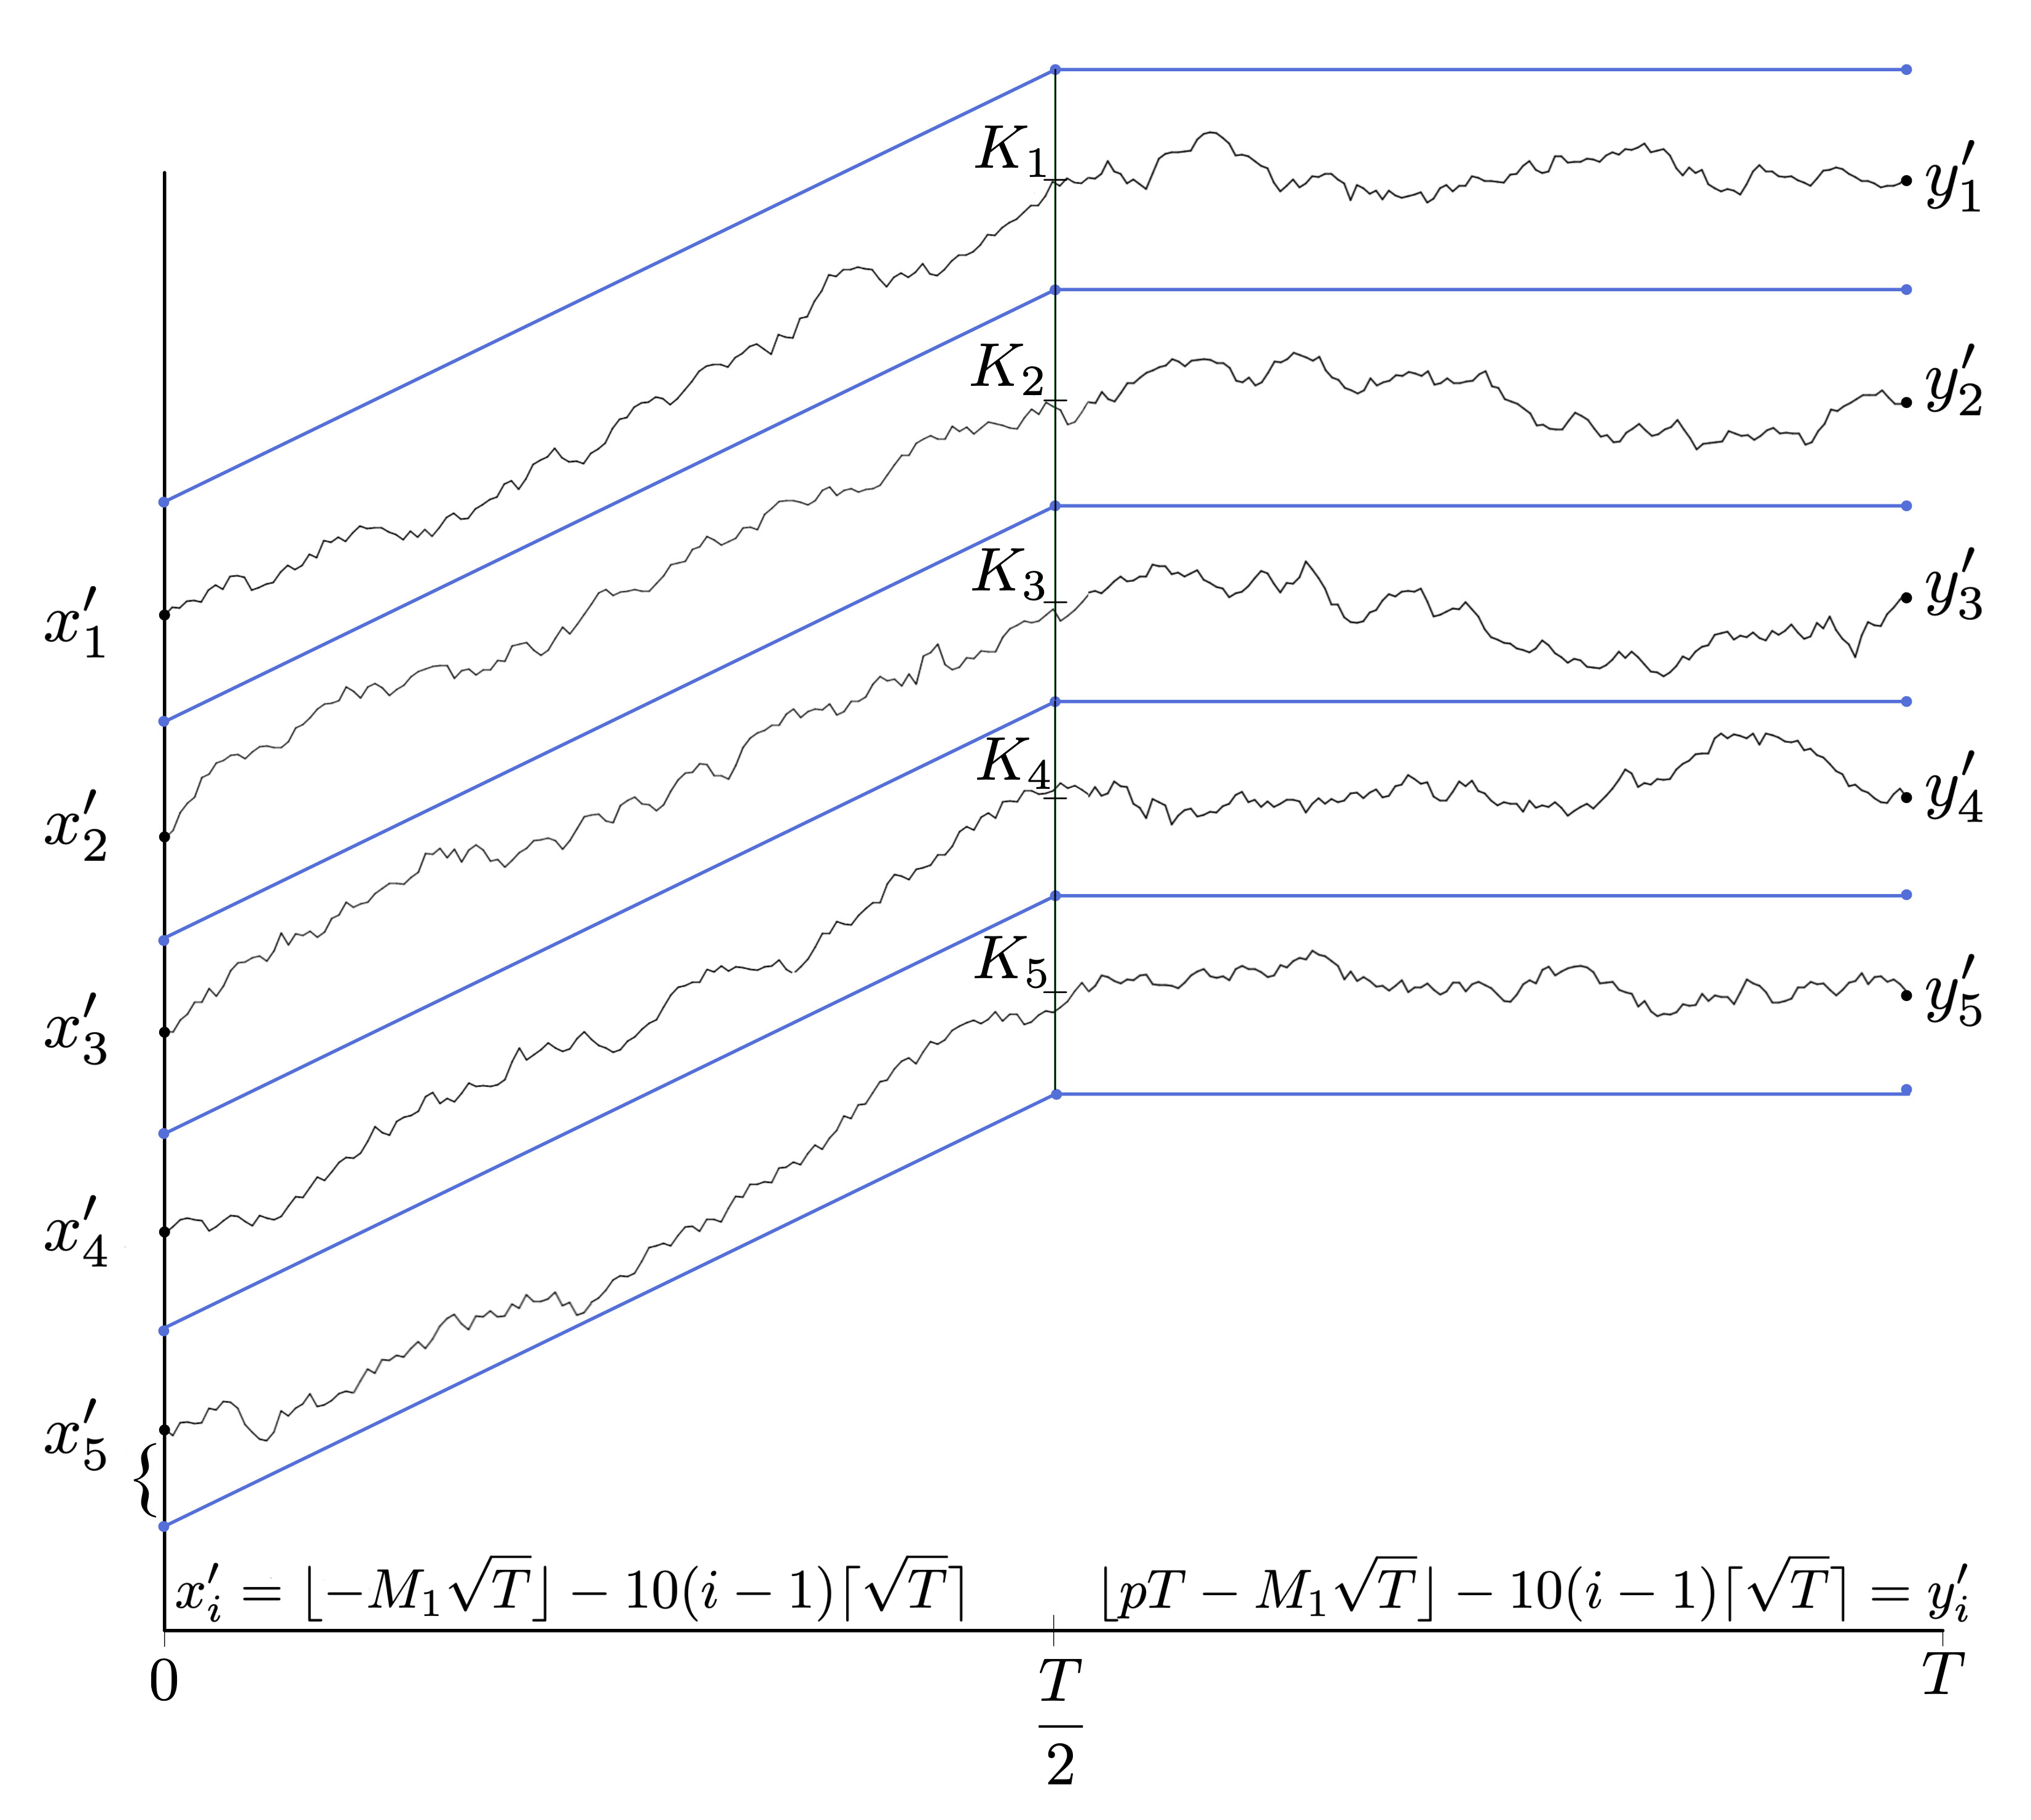
\includegraphics[scale=0.6]{graphics/Lemma320.jpg}
	\caption{Sketch of the argument for Lemma \ref{prob19}: We use Lemma \ref{MCLxy} to lower the entry and exit data $\vec{x},\vec{y}$ of the curves to $\vec x\,'$ and $\vec y\,'$. The event $E$ occurs when each curve lies within the blue bounding lines shown in the figure. We then use strong coupling with Brownian bridges via Theorem \ref{KMT} and bound the probability of the bridges remaining within the blue windows.}
\end{figure}
	Let $\mathbb{P}$ be a probability space supporting a random variable $\ell^{(T,z)}$ with law $\mathbb{P}^{0,T,0,z}$ coupled with a Brownian bridge $B^\sigma$ with variance $\sigma^2$, as in Theorem \ref{KMT}. Then the expression in \eqref{19gibbs} is bounded below by
	\begin{equation}\label{19BB}
	\begin{split}
	& \mathbb{P}^{0,T,0,z}_{Ber}\bigg(\left|\ell(T/2)-pT/2-(M+M_1+5)\sqrt{T}\right|\leq 2\sqrt{T} - 5\quad\mathrm{and}\\
	&\qquad \sup_{s\in[0,T/2]}\left|\ell(s)-ps-\frac{M+M_1+5}{\sqrt{T}/2}\,s\right| \leq 3\sqrt{T} - 1 \quad\mathrm{and}\\
	&\qquad \sup_{s\in[T/2,T]}\left|\ell(s)-ps-(M+M_1+5)\sqrt{T}+\frac{M+M_1+5}{\sqrt{T}/2}(s-T/2)\right| \leq 3\sqrt{T} - 1 \bigg) \geq\\
	& \mathbb{P}\bigg(\left|\sqrt{T}\,B^\sigma_{1/2} - (M+M_1+5)\sqrt{T}\right|\leq \sqrt{T} \quad\mathrm{and}\\
	&\qquad\sup_{s\in[0,T/2]}\left|\sqrt{T}\,B^\sigma_{s/T}-(M+M_1+5)\sqrt{T}\cdot\frac{s}{T/2}\right| \leq 2\sqrt{T}\quad\mathrm{and}\\
	&\qquad \sup_{s\in[T/2,T]}\left|\sqrt{T}\,B^\sigma_{s/T}-(M+M_1+5)\sqrt{T}\cdot\frac{T-s}{T/2}\right| \leq 2\sqrt{T} \bigg) -  \mathbb{P}\left(\Delta(T,z) > \sqrt{T}/2\right).
	\end{split}
	\end{equation}
	Note that $B^\sigma_{1/2}$ is a centered Gaussian random variable with variance $p(1-p)/4 = \sigma^2(1/2)(1-1/2)$. Writing $\xi = B^\sigma_{1/2}$, it follows from Lemma \ref{2bridges} that there exist independent Brownian bridges $B^1,B^2$ with variance $\sigma^2/2$ so that $B^\sigma_s$ has the same law as $\frac{s}{T/2}\xi + B^1_{2s/T}$ for $s\in[0,T/2]$ and $\frac{T-s}{T/2}\xi + B^2_{(2s-T)/T}$ for $s\in[T/2,T]$. The first term in the last expression in \eqref{19BB} is thus equal to
	\begin{equation}\label{prob19split}
	\begin{split}
	&\mathbb{P}\bigg(|\xi - (M+M_1+5)|\leq 1 \quad\mathrm{and} \sup_{s\in[0,T/2]}\left|B^1_{s/T}-(M+M_1+5-\xi)\cdot\frac{s}{T/2}\right| \leq 2 \quad \mathrm{and}\\
	&\qquad  \sup_{s\in[T/2,T]}\left|B^2_{(2s-T)/T}-(M+M_1+5-\xi)\cdot\frac{T-s}{T/2}\right| \leq 2 \bigg) \geq \\
	& \mathbb{P}\bigg(|\xi - (M+M_1+5)|\leq 1 \quad\mathrm{and} \sup_{s\in[0,T/2]}\big|B^1_{2s/T}\big| \leq 1 \qquad \mathrm{and}\quad \sup_{s\in[T/2,T]}\big|B^2_{(2s-T)/T}\big| \leq 1 \bigg) =\\
	& \mathbb{P}\Big(|\xi-(M+M_1+5)|\leq 1\Big)\cdot \mathbb{P}\bigg(\sup_{s\in[0,T/2]} \big|B^1_{2s/T}\big|\leq 1\bigg)\cdot \mathbb{P}\bigg(\sup_{s\in[0,T/2]} \big|B^2_{(2s-T)/T}\big|\leq 1\bigg) \geq\\
	& \left(1-2e^{-4/p(1-p)}\right)^2 \int_{M+M_1+4}^{M+M_1+6} \frac{e^{-2\xi^2/p(1-p)}}{\sqrt{\pi p(1-p)/2}}\,d\xi \geq\\
	& \frac{2\sqrt{2}\,e^{-2(M+M_1+6)^2/p(1-p)}}{\sqrt{\pi p(1-p)}}\,\big(1-2e^{-4/p(1-p)}\big)^2.
	\end{split}
	\end{equation}
	In the fourth line, we used the fact that $\xi$, $B^1_\cdot$, and $B^2_\cdot$ are independent, and in the second to last line we used Lemma \ref{BBmax}. Since $|z-pT|\leq (M_1+1)\sqrt{T}$, Lemma \ref{Cheb} allows us to choose $T$ large enough so that $\mathbb{P}(\Delta(T,z) > \sqrt{T}/2)$ is less than 1/2 the expression in the last line of \eqref{prob19split}. Then in view of \eqref{19gibbs} and \eqref{19BB}, we conclude \eqref{19ineq}.
	
\end{proof}

We now state a weak convergence result, whose proof we postpone until Section \ref{Section9}, in particular in Propositions \ref{WeakConvDistinct} and \ref{WeakConvCollide}.

\begin{lemma}\label{prob17}
Fix $p,t\in(0,1)$, $k\in\mathbb{N}$, $\vec a, \vec b\in \mathfrak{W}_k$.  Suppose that $\vec{x}^{T}=(x_{1}^{T},\dots,x_{k}^{T})$ and $\vec{y}^{T}=(y_{1}^{T},\dots,y_{k}^{T})$ are two sequences in $\mathfrak{W}_k$ such that for $i\in \llbracket 1,k\rrbracket$, $$\lim_{T\rightarrow\infty}\frac{x_{i}^{T}}{\sqrt{T}}=a_{i} \quad \text{and} \quad \lim_{T\rightarrow\infty}\frac{y_{i}^{T}-pT}{\sqrt{T}}=b_{i}.$$  Let $(Q_1^T,\dots,Q_k^T)$ have law $\mathbb{P}^{0,T,\vec{x}^{T},\vec{y}^{T}}_{avoid,Ber}$, and define the sequence $\{Z^T\}$ of random $k$-dimensional vectors by $$Z^{T}=\left(\frac{Q_{1}^T(tT)-ptT}{\sqrt{T}},\dots,\frac{Q_{k}^T(tT)-ptT}{\sqrt{T}}\right).$$ Then as $T\to\infty$, $Z^{T}$ converges weakly to a random vector $\hat Z$ on $\mathbb{R}^k$ with a probability density $\rho$ supported on $W_k^\circ$.
\end{lemma}

The convergence result in Lemma \ref{prob17} allows us to prove the following lemma, which roughly states that if the entrance and exit data of a sequence of avoiding Bernoulli line ensembles remain in compact windows, then with high probability the curves of the ensemble will remain separated from one another at each point by some small positive distance.

\begin{lemma}\label{prob 20}
Fix $p,t\in (0,1)$ and $ k\in \mathbb{N}$. Suppose that $\vec x\,^T=(x_1^T,\dots, x_k^T)$, $\vec y\,^T=(y_1^T,\dots , y_k^T)$ are elements of $\mathfrak{W}_k$ such that $T\geq y_i^T-x_i^T\geq 0$ for $i\in \llbracket 1,k\rrbracket$. Then for any $M_1,M_2>0$ and $\epsilon>0$ there exists $W_7\in\mathbb{N}$ and $\delta>0$ depending on $p,k,M_1,M_2$ such that if $T\geq W_7$, $|x_i^T|\leq M_1\sqrt{T}$ and $|y_i^T-pT|\leq M_2\sqrt{T}$, then 
\[
\pr^{0,T,\vec x^T, \vec y^T}_{avoid,Ber}\left(\min_{1\leq i\leq k-1} \big[Q_i(tT)-Q_{i+1}(tT)\big]<\delta\sqrt{T}\right)<\epsilon.
\]
\end{lemma}
\begin{proof}
	We prove the claim by contradiction. Suppose there exist $M_1,M_2,\epsilon>0$ such that for any $W_7\in \mathbb{N}$ and $\delta>0$ there exists some $T\geq W_7$ with
	\[
	\pr^{0,T,\vec x^T,\vec y^T}_{avoid, Ber}\left(\min_{1\leq i\leq k-1}\big[Q_i(tT)-Q_{i+1}(tT)\big]<\delta\sqrt{T}\right)\geq \epsilon.
	\]
	Then we can obtain sequences $T_n$, $\delta_n>0$, $T_n \nearrow \infty$, $\delta_n \searrow 0$, such that for all $n$ we have  
	\[
	\pr^{0,T,\vec x\,^{T_n},\vec y\,^{T_n}}_{avoid, Ber}\left(\min_{1\leq i\leq k-1}\left[\frac{Q_i(tT_n)-Q_{i+1}(tT_n)}{\sqrt{T_n}}\right]<\delta_n\right)\geq \epsilon.
	\]
	Since $|x_i^{T_n}|<M_1\sqrt{T_n}$ and $|y_i^{T_n}-pT_n|\leq M_2\sqrt{T_n}$ for $1\leq i\leq k$, the sequences $\{\vec{x}\,^{T_n}/\sqrt{T_n}\}$, $\{(\vec{y}\,^{T_n}-pT_n)/\sqrt{T_n}\}$ are bounded in $\mathbb{R}^k$. It follows that there is a subsequence $\{T_{n_m}\}$ such that \[
	\frac{\vec{x}\,^{T_{n_m}}}{\sqrt{T_{n_m}}} \longrightarrow \vec x, \quad
	\frac{\vec{y}\,^{T_{n_m}}-pT_{n_m}}{\sqrt{T_{n_m}}} \longrightarrow \vec y
	\] 
	as $m\to\infty$ (see \cite[Theorem 3.6]{Rudin}). Denote $$Z_i^m =\frac{Q_i(tT_{n_m})-ptT_{n_m}}{\sqrt{T_{n_m}}}.$$ Fix $\delta > 0$ and choose $M$ large enough so that if $m\geq M$ then $\delta_m < \delta$. Then for $m\geq M$ we have
	\begin{equation}\label{prob20inf}
	\epsilon\leq \liminf_{m\to\infty}\pr\left(\min_{1\leq i\leq k-1} \big[Z_i^m-Z_{i+1}^m\big] < \delta_{n_m}\right) \leq \liminf_{m\to\infty}\pr\left(\min_{1\leq i\leq k-1} \big[ Z_i^m-Z_{i+1}^m\big] \leq\delta\right).
	\end{equation}
	Now by Lemma \ref{prob17}, $(Z_1^m,\dots, Z_k^m)$ converges weakly to a random vector $\hat Z$ on $\mathbb{R}^k$ with a density $\rho$. It follows from the portmanteau theorem \cite[Theorem 3.2.11]{Durrett} applied with the closed set $K=[0,\delta]$ that
	\begin{equation}\label{prob20sup}
	\limsup_{m\to\infty }\pr\left(\min_{1\leq i\leq k-1} \big[Z_i^m-Z_{i+1}^m\big]\in K\right)\leq \pr\left(\min_{1\leq i\leq k-1} \big[\hat Z_i-\hat Z_{i+1}\big]\in K\right).
	\end{equation}
	Combining (\ref{prob20inf}) and (\ref{prob20sup}), we obtain
	\begin{equation}\label{eq:ineq}
	\epsilon\leq \pr\left(0 \leq \min_{1\leq i\leq k-1} \big[\hat Z_i-\hat Z_{i+1}\big]\leq\delta\right)\leq \sum_{i=1}^{k-1}\pr\left(0 \leq \hat Z_i-\hat Z_{i+1}\leq \delta\right).
	\end{equation}
	To conclude the proof, we find a $\delta$ for which \eqref{eq:ineq} cannot hold. For $\tilde\eta\geq 0$ put
	\[
	E_i^{\tilde\eta} = \{\vec{z} \in\mathbb{R}^k : 0 \leq z_i-z_{i+1}\leq\tilde\eta\}.
	\] 
	For each $i\in\llbracket 1, k-1\rrbracket$ and $\eta > 0$, we have
	\begin{equation}\label{eq:integral}
	\mathbb{P}\left(0 \leq \hat{Z}_i - \hat{Z}_{i+1} \leq \eta\right) = \int_{\mathbb{R}^k} \rho\cdot\mathbf{1}_{E_i^\eta}\,dz_1\cdots dz_k.
	\end{equation}
	Clearly $\rho \cdot \mathbf{1}_{E_i^\eta} \to \rho \cdot \mathbf{1}_{E_i^0}$ pointwise as $\eta \to 0$, and $E_i^0 = \{\vec{z} \in\mathbb{R}^k : z_i = z_{i+1}\}$ has Lebesgue measure 0. Thus $\rho\cdot\mathbf{1}_{E_i^\eta} \to 0$ a.e. as $\eta\to 0$. Since $|\rho\cdot\mathbf{1}_{E_i^\eta}| \leq \rho$ and $\rho$ is integrable, the dominated convergence theorem \cite[Theorem 1.34]{RudinRCA} and \eqref{eq:integral} imply that
	\begin{equation*}
	\mathbb{P}\left(0 \leq \hat{Z}_i - \hat{Z}_{i+1} \leq \eta\right) \longrightarrow  0
	\end{equation*}
	as $\eta\to 0$.	Thus for each $i\in\llbracket 1,k-1\rrbracket$ and $\epsilon > 0$ we can find an $\eta_i > 0$ such that $0<\eta \leq \eta_i$ implies $\mathbb{P}(0 \leq \hat{Z}_i - \hat{Z}_{i+1} \leq \eta)<\epsilon/(k-1)$. Putting $\delta=\min_{1\leq i\leq k-1}\eta_i$ we find that 
	\begin{equation*}
	\sum_{i=1}^{k-1}\pr\left( 0 \leq \hat Z_i-\hat Z_{i+1}\leq\delta \right) < \epsilon,
	\end{equation*}
	contradicting \eqref{eq:ineq} for this choice of $\delta$.
	
\end{proof}
